%%%%%%%%%%%%%%%%%%%%%%%%%%%%%%%%%%%%%%%%%%%%%%%%%%%%%%%%%%%%%%%%%%%%%%%
% This document is based on the template: Large Colored Title Article %
%                                         Version 1.1 (25/11/12)      %
%                                                                     %
% The template was downloaded from: http://www.LaTeXTemplates.com     %
%                                                                     %
% Original author:                                                    %
% Frits Wenneker (http://www.howtotex.com)                            %
%                                                                     %
% License:                                                            %
% CC BY-NC-SA 3.0 (http://creativecommons.org/licenses/by-nc-sa/3.0/) %
%                                                                     %
% Authors of this version:                                             %
% Adrian Quintas Garcia              %
% Yuriy Mischenko              %
%                                                                     %
% Original licensing terms are maintained                             %
%%%%%%%%%%%%%%%%%%%%%%%%%%%%%%%%%%%%%%%%%%%%%%%%%%%%%%%%%%%%%%%%%%%%%%%

%----------------------------------------------------------------------------------------
%	PACKAGES AND OTHER DOCUMENT CONFIGURATIONS
%----------------------------------------------------------------------------------------

\documentclass[DIV=calc,paper=a4,fontsize=11pt,onecolumn]{scrartcl}	 % A4 paper and 11pt font size

\usepackage[galician]{babel} % Galician language/hyphenation
\usepackage[utf8]{inputenc}
\usepackage[protrusion=true,expansion=true]{microtype} % Better typography
\usepackage{amsmath,amsfonts,amsthm} % Math packages
\usepackage[svgnames]{xcolor} % Enabling colors by their 'svgnames'
\usepackage[hang,small,labelfont=bf,up,textfont=it,up]{caption} % Custom captions under/above floats in tables or figures
\usepackage{booktabs} % Horizontal rules in tables
\usepackage{fix-cm}	 % Custom font sizes - used for the initial letter in the document

\usepackage{sectsty} % Enables custom section titles
\allsectionsfont{\usefont{OT1}{phv}{b}{n}} % Change the font of all section commands

\usepackage{fancyhdr} % Needed to define custom headers/footers
\pagestyle{fancy} % Enables the custom headers/footers
\usepackage{lastpage} % Used to determine the number of pages in the document (for "Page X of Total")

% Headers - all currently empty
\lhead{}
\chead{}
\rhead{}

% Footers
\lfoot{\textsc{vvs-monitorización-probas}}
\cfoot{}
\rfoot{\footnotesize Páxina \thepage\ de \pageref{LastPage}} % "Page 1 of 2"

\renewcommand{\headrulewidth}{0.0pt} % No header rule
\renewcommand{\footrulewidth}{0.4pt} % Thin footer rule

\definecolor{UDC}{RGB}{206,0,124}
\definecolor{DarkUDC}{rgb}{0.75,0.75,0.75}
\definecolor{LightUDC}{RGB}{128,128,128}

\usepackage{lettrine} % Package to accentuate the first letter of the text
\newcommand{\initial}[1]{ % Defines the command and style for the first letter
\lettrine[lines=3,lhang=0.3,nindent=0em]{
\color{UDC}
{\textsf{#1}}}{}}

%----------------------------------------------------------------------------------------
%	TITLE SECTION
%----------------------------------------------------------------------------------------

\usepackage{titling} % Allows custom title configuration

\newcommand{\HorRule}{\color{UDC} \rule{\linewidth}{1pt}} % Defines the pink horizontal rule around the title

\pretitle{\vspace{-30pt} \begin{flushleft} \HorRule \fontsize{20}{20} \usefont{OT1}{phv}{b}{n} \color{DarkUDC} \selectfont} % Horizontal rule before the title

\title{MONITORIZACIÓN DE PROBAS} % Your article title

\posttitle{\par\end{flushleft}\vskip 0.5em} % Whitespace under the title

\preauthor{\begin{flushleft}\large \lineskip 0.5em \usefont{OT1}{phv}{b}{sl} \color{DarkUDC}} % Author font configuration

\author{Título proxecto: Práctica \\
	Ref. proxecto: Verificación y validación de software}

\postauthor{\footnotesize \usefont{OT1}{phv}{m}{sl} \color{Black} % Configuration for the institution name
\par\end{flushleft}\HorRule} % Horizontal rule after the title

\date{\sffamily Validación e Verificación de Software} % Add a date here if you would like one to appear underneath the title block

%----------------------------------------------------------------------------------------

\usepackage{graphicx}
\usepackage{hyperref}
\hypersetup{colorlinks=true,
            allcolors=UDC}

\usepackage{array}
\usepackage{colortbl}

%----------------------------------------------------------------------------------------

\newcommand{\hint}[1]{\begin{quote}\itshape #1 \end{quote}}

%----------------------------------------------------------------------------------------

\begin{document}

\maketitle % Print the title
\thispagestyle{fancy} % Enabling the custom headers/footers for the first page 

%----------------------------------------------------------------------------------------
%	ABSTRACT
%----------------------------------------------------------------------------------------

\vspace*{1cm}

\begin{center}
\small \sffamily
\begin{tabular}{c|c|c}
Data de aprobación & Control de versións & Observacións \\ \hline
& & \\ \hline
& & \\ \hline
& & \\
\end{tabular}
\end{center}

\clearpage

%----------------------------------------------------------------------------------------
%	ARTICLE CONTENTS
%----------------------------------------------------------------------------------------

\section{Contexto}

\hint{El proyecto presenta un único plan de pruebas.
	El desarrollo implica dos iteraciones, una primera iteración con una batería de pruebas de funcionalidades, y una segunda iteración con 
	diversas utilidades de terceros para apoyar las pruebas tanto funcionales como no funcionales.}

\section{Estado actual}

\hint{ Todas las funcionalidades requeridas para el sistema han sido implementadas desde la primera iteración del proyecto.}

\subsection{Funcionalidades}

\hint{ 
			\begin{enumerate}
				\item Alta de servidor: 1 test.
				\item Baja de servidor: 2 tests.
				\item Buscar contenido en el servidor: 4 tests.
				\item Agregar contenido en el servidor: 4 tests.
				\item Eliminar contenido en el servidor: 1 test.
				\item Obtener lista de reproducción de contenido: 3 tests.
				\item Buscar contenido dentro de emisoras: 1 test.
				\item Eliminar contenido dentro de emisoras: 1 test.
			\end{enumerate}
	}

\section{Rexisto de probas}

\hint{
	Las pruebas realizadas cubren poco más de 90 por ciento de cobertura del código. Si se añaden nuevas funcionalidades o clases, deben crear nuevos tests para esas modificaciones.
	}

\section{Rexistro de erros}

\hint{No se han encontrado errores.}

\section{Estatísticas}

\hint{
  \begin{itemize}
    \item Debido a la calidad del código, no se han encontrado errores durante las pruebas.
    \item Las pruebas se han perfilado para cubrir el mayor número de casos posibles.
    \item Los únicos errores encontrados fueron relacionados con los puertos de los servidores, pero nunca ninguno relacionado con el código.
    \item Debido a la ausencia de errores, no se han abierto ningún ticket de éstos.
    \item Tanto el código como los tests implementados cubren una cantidad más que aceptable de funcionalidades y código, confirmando la robustez del proyecto.
    \item La media de cobertura de código en las clases de implementación es 86,25 por ciento.
  \end{itemize}}

\section{Outros aspectos de interese}

\hint{
	\begin{itemize}
		\item Gráfica de cobertura.
		
		\begin{center}
		   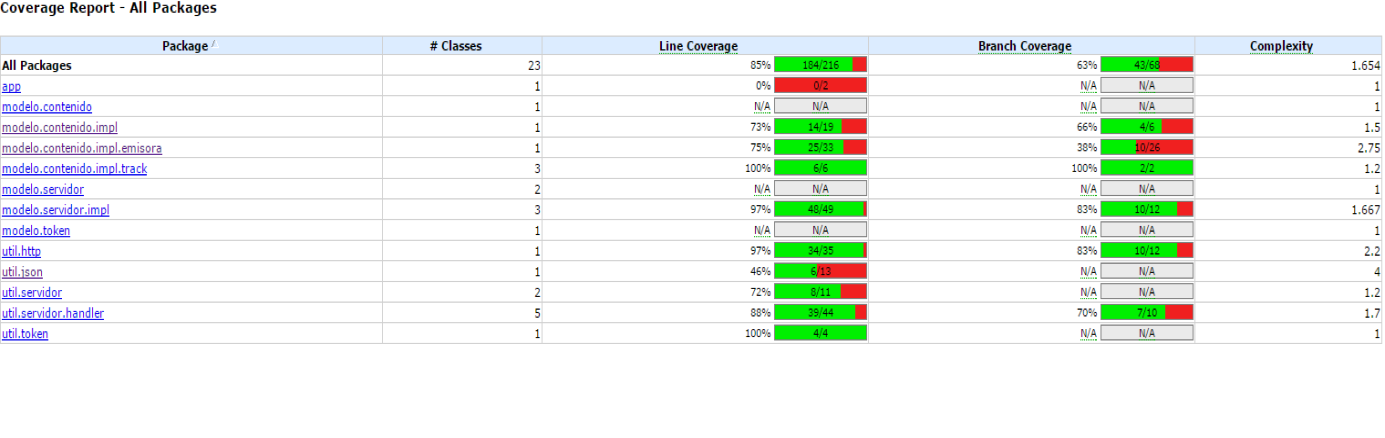
\includegraphics[scale=0.5,center]{images/cobertura.png}
	    \end{center}
	
		\item JETM, resumen de performance.
		
		\begin{center}
			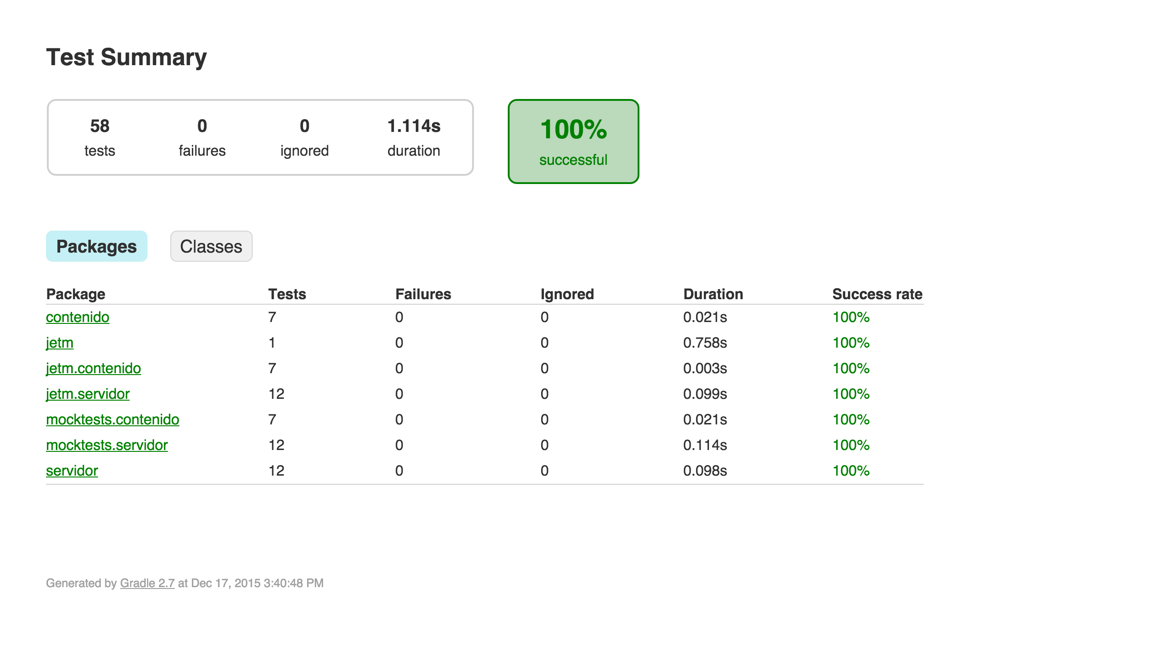
\includegraphics[scale=0.7,center]{images/jetm_summary.png}
		\end{center}		
		
		\begin{center}
			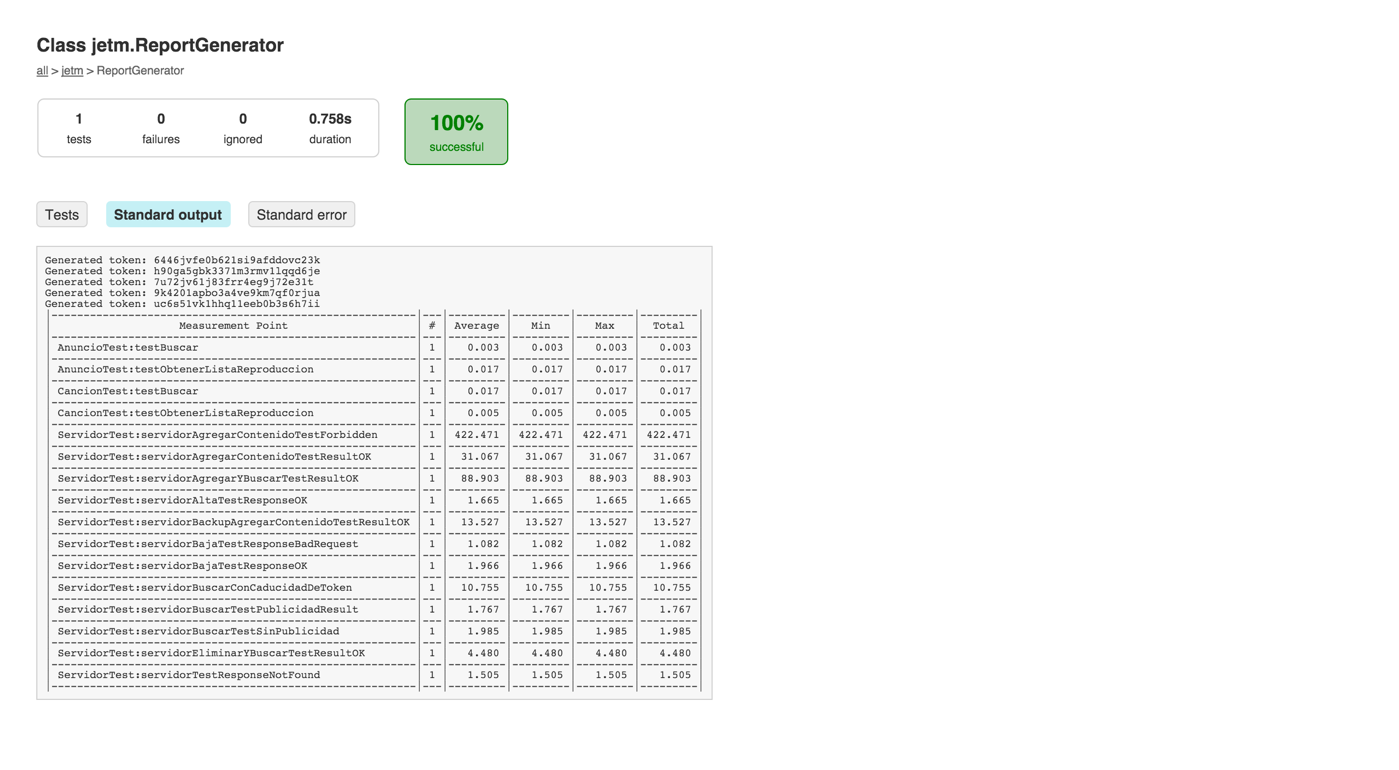
\includegraphics[scale=0.7,center]{images/jetm_details.png}
		\end{center}				
		
		\item Herramientas de evaluación de calidad del código presentan algunos consejos para mejorar la implementación, y sus consejos deben ser analizados para implementar en la próxima iteración del proyecto. 
	\end{itemize}}

\end{document}
